% 2004 年全国卷Ⅳ理科第 20 题：四棱锥立体几何图
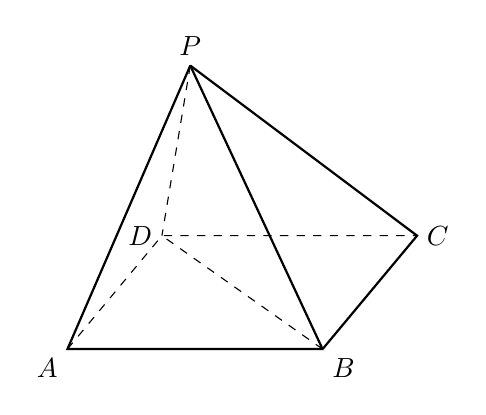
\begin{tikzpicture}[>=stealth,scale=1.2]
  % Coordinates
  \coordinate (A) at (-1.5,-0.8);
  \coordinate (B) at (1.2,-0.8);
  \coordinate (C) at (2.2,0.4);
  \coordinate (D) at (-0.5,0.4);
  \coordinate (P) at (-0.2,2.2);

  % Solid edges
  \draw[thick] (P) -- (A) -- (B) -- (C) -- (P);
  \draw[thick] (P) -- (B);

  % Dashed edges
  \draw[dashed] (A) -- (D) -- (C);
  \draw[dashed] (P) -- (D);
  \draw[dashed] (B) -- (D);

  % Labels
  \node[below left] at (A) {$A$};
  \node[below right] at (B) {$B$};
  \node[right] at (C) {$C$};
  \node[left] at (D) {$D$};
  \node[above] at (P) {$P$};
\end{tikzpicture}
